\documentclass[11pt]{article}

\usepackage[top=1in, bottom=1in, left=1in, right=1in]{geometry}
\usepackage{amsfonts}
\usepackage{graphicx}
\usepackage{float}
\usepackage[utf8]{inputenc}
\usepackage[section]{placeins}
\usepackage{abstract}
\usepackage{amsmath}
\usepackage{amsfonts}
\usepackage{amssymb}
\usepackage{enumitem}
\renewcommand{\abstractnamefont}{\normalfont\bfseries} 
\renewcommand{\abstracttextfont}{\normalfont} 
\numberwithin{equation}{section}
\newcommand{\argmax}{\operatornamewithlimits{argmax}}

\begin{document}

\title{DMUU Project Report}
\author{\begin{tabular}{cc}
Roland Hellström & Sebastian Ånerud \\
XXXXXX-xxxx & 910407-5958 \\
asdf.comasd@ & anerud@student.chalmers.se
\end{tabular}}
\date{\today}
\maketitle

\begin{flushleft}

\section{Introduction}

very much introductory. so amaze. wow.

\section{Method}

very much methods. so amaze. wow.

\section{Results}

very much results. so amaze. wow. \newline 

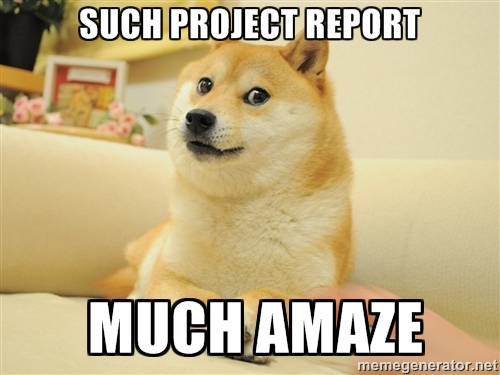
\includegraphics[scale=1]{DOGE}

\section{Discussion}

very much discuss. so amaze. wow.

\section{Conclusion}

very much conclude. so amaze. wow.

\end{flushleft}

\end{document}